\setcounter{page}{1}
\section*{Zielsetzung}

\section{Theorie}
\subsection{CDefinition des Vakuums}
Ein Raum ohne Materie wird Vakuum genannt. Als physikalische Messgröße zur Charakterisierung
des Vakuums wird der Gasdruck $p$ verwendet, der durch Stöße von Gasmolekülen mit den Wänden eines Bahälters
entsteht. Da sich in einem Behälter allgemein mehrere Gase befinden, setzt sich der Druck aus der Summe aller
Partialdrücke $p\ua{i}$ zusammen.
In Tabelle \ref{tab: vakuumbegriffe} sind Einteilungen des Vakuumbegriffs in Abhängigkeit vom
Druck $p$ aufgeführt.
\begin{table}
  \centering
  \begin{tabular}{l l}
    \toprule
    {Vakuumtyp} & {Druckintervall $p/\si{\milli\bar}$} \\
    \midrule
    Grobvakuum &  $[\num{300},\,\num{1}]$ \\
    Feinvakuum &  $(\num{1},\,\num{e-3}]$ \\
    Hochvakuum &  $(\num{e-3},\,\num{e-7}]$ \\
    Ultrahochvakuum &  $(\num{e-7},\,\num{e-12}]$ \\
    \bottomrule
  \end{tabular}
  \caption{Begriffliche Einteilungen des Vakuumbegriffs in Abhängigkeit vom Gasdruck $p$ \cite{dem1}.}
  \label{tab: vakuumbegriffe}
\end{table}
Eine weitere wichtige Größe zur Diskussion von Evakuierungsprozessen ist die mittlere freie
Weglänge $\Lambda$. Diese ist definiert als die durchschnittliche Länge zwischen zwei Stößen
eines Gasmoleküls. Für eine gemäß Maxwell und Boltzmann verteilte Geschwindigkeit der Gasmoleküle kann
folgende Formel für $\Lambda$ angegeben werden
\begin{equation}
  \Lambda = \frac{1}{\sqrt{2}\pi n D^2}.
\end{equation}
Mit der Stoffmenge $n$ und dem Moleküldurchmesser $D$. Mit fallendem Druck wächst die mittlere freie
Weglänge an und erreicht den theoretischen Wert $\infty$ im idealen Vakuum.

\subsection{Erzeugung des Vakuums}
Eine Apperatur zur Erzeugung eines Vakuums wird als Vakuumpumpe bezeichnet. Diese besitzt ein
Saugvermögen $S$, das den Gasvolumendurchfluss zwischen Pumpe und Rezipient \footnote{Der Hohlraum, in dem das Vakuum erzeugt werden soll.}
angibt
\begin{equation}
  S = \frac{\dif{}}{\dif{t}} V.
\end{equation}
Das Saugvermögen wird oft bezogen auf das Einheitsvolumen in $[S\ua{L}] = \si{\pascal \per \second}$ angegeben.
Das Produkt aus Druck $p$ und Saugvermögen $S$ wird als Saugleistung $S\ua{L}$ definiert
\begin{equation}
  S\ua{L} = p S = L \Delta p ,
\end{equation}
Die Saugleistung ist proportional zu einer erzeugten Druckdifferenz $\Delta p$,
wobei der proportionalitätsfaktor $L$ als Leitwert bezeichnet wird und stark vom verwendeten Bauteil abhängt.
Der Kehrwert des Leitwertes wird Strömungswiderstand $R$ genannt. Der Gesamtsströmungswiderstand einer Leitungsreihe
stellt sich als Summe der einzelnen auftrenden Widerstände dar. Daher gilt für das effektive Saugvermögen $S\ua{eff}$ am Rezipienten
\begin{equation}
 \frac{1}{S\ua{eff}} = \frac{1}{S_0} + \frac{1}{L}.
 \label{eq: effektives_saugvermögen}
\end{equation}
Mit dem Saugvermögen $S_0$ ohne Leitungen (Herstellerangabe).

Der erzeugte Strom durch ein Rohr zwischen Pumpe und Rezipient ist stark von der mittleren freien Weglänge
und damit vom Typ des Vakuums abhängig. Ist $\Lambda$ wesentlich
kleiner als der Durchmesser der verwendeten Bauteile, so kann von laminaren Strömungen ausgegangen werden. Gilt andersherum
$\Lambda >> d$, so werden Stöße der Moleküle mit den Wänden relevant. In diesem Fall wird von einer molekularen Strömung gesprochen.


\subsubsection{Pumpentypen}



\subsection{Zeitlicher Verlauf des Drucks}
Zur Herleitung eines Zusammenhangs für den zeitlichen Verlauf des Drucks $p(t)$, der durch eine Pumpe
hervorgerufen wird, werden im Folgenden einige vereinfachende Annahmen getroffen. Zunächst soll das
verwendete Gas der idealen Gasgleichung genügen
\begin{equation}
  p V = n R T.
  \label{eq: ideale_gasgleichung}
\end{equation}
Mit Systemvolumen $V$ und Temperatur $T$. Geht man davon aus, dass das System bestehend aus
Pumpe und Rezipient ideal abgeschlossen ist, so gilt
\begin{equation}
  \frac{\dif{}}{\dif{t}}(n R T ) = 0.
\end{equation}
Und damit das Boylesche Gesetz
\begin{equation}
  0 = \dot{p}V  + p\dot{V}.
\end{equation}
Die zeitliche Änderung des Volumens wird als Saugvermögen $S$ der Pumpe angenommen. Es ergibt sich eine Differentialgleichung für $p(t)$
\begin{equation}
  \dot{p} = - \frac{S}{V} p,
\end{equation}
die durch Separation der Variablen gelöst werden kann. Zur Zeit $t = 0$ soll der Druck einen Wert $p_0$ haben und für große
Zeiten soll die Funktion gegen einen Grenzwert $p\ua{G} > 0$ laufen. Letzteres wird durch eine Inhomogenität in der DGL berücksichtigt
\begin{equation}
  \dot{p}(t) = - \frac{S}{V} \left(p(t) + p\ua{G}\right).
\end{equation}
Hieraus ergibt sich schließlich
\begin{equation}
  p(t) = (p_0 - p\ua{E})\exp\left(- \frac{S}{V} t \right) + p\ua{G}.
  \label{eq: evakuierungskurve}
\end{equation}
Eine grafische Darstellung des theoretischen Druckverlaufs $p(t)$ befindet sich in Abbildung~\ref{fig: theo_p_t}.
\begin{figure}[h]
  \centering
  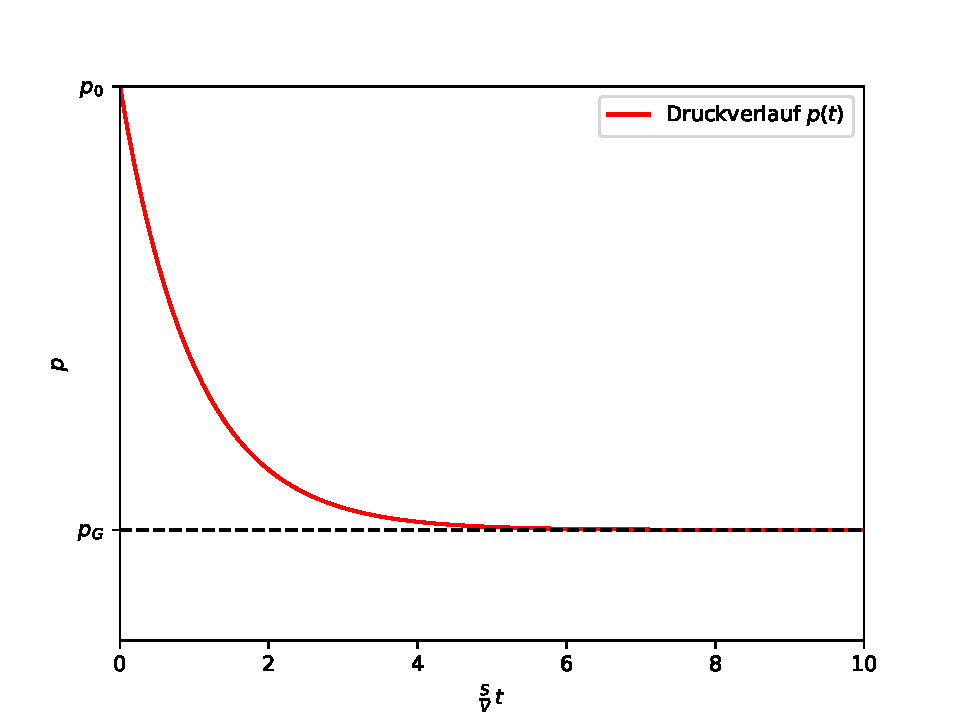
\includegraphics[width = 0.7\textwidth]{theorie_plots/theo_p.pdf}
  \caption{Grafische Darstellung der Funktion $p(t)$ gemäß Gleichung \eqref{eq: evakuierungskurve}.}
  \label{fig: theo_p_t}
\end{figure}

Der Grenzwert $p\ua{G}$ tritt auf, da eine reale Apparatur nicht ideal abgedichtet werden kann. Pro Zeiteinheit
strömt ein Menge an Gas durch auftretende Lecks in den Rezipienten, was analog zur Saugleistung
die Definition einer Leckrate $Q$ nahe legt
\begin{equation}
  Q = V \frac{\dif{}}{\dif{t}} p.
\end{equation}
Der Gleichgewichtsdruck stellt sich ein, wenn Leckrate und Saugleistung einander ausgleichen
\begin{equation}
  p\ua{G} S\ua{eff} =  V \frac{\dif{}}{\dif{t}} p \, \Leftrightarrow \,
  S\ua{eff} =  \frac{V}{p\ua{G}} \frac{\dif{}}{\dif{t}} p
  \label{eq: saugvermögen_leckrate}
\end{equation}
